\subsection{Isosurface extraction\pavol{update plot text to isosurface}}
\label{sec:isocontour}
Another common visualization task is display of boundaries, usually done using isosurfaces. For example,
isosurface of OH concentration can separate burning and extinguished regions in a combustion simulation or
organs can be extracted from medical imaging by threshold on a CT scalars. Moreover, topological methods such as Reeb Graph is
defined by contracting isosurfaces to a point and building the structure from equivalence classes of isosurfaces.
Extraction of isosurfaces is therefore an essential task in any
visualization and analysis system. We thus study the characteristics of bit streams that
minimize errors in the reconstructed isosurfaces and compare those streams quantitatively and qualitatively.

\pavol{potentially weak point as we do not use any standard error metric here; is the relative surface area fudge
necessary for higher resolution datasets?}
As before, we begin by defining an error metric to compare isosurfaces. Commonly used metric is a Hausdorff
distance that measures the shortest path from a point on one surface to the other, and then taking maximum
of all those paths. Unfortunately, the distance is not very robust and can vary drastically with minor changes
in the surfaces. For example, a single perturbation in one of the two surfaces
can result in a large distance even when the surfaces are close to identical. Therefore, we use a number of
misclassified voxels as our distance which can be computed by counting all voxels that are either in surface $S_1$
and not surface $S_2$ or the other way. \pavol{not sure if following is needed}We have found that if the error caused by
switching off a chunk is too small (in orders of sub-pixel/sub-voxel), then the importance of the
chunk cannot be properly measured. We therefore amend the error metric by adding to it the relative
difference in area between two isosurfaces. This relative difference is, most of the time, a number
between $0$ and $1$, computed by the formula $|A(S_1)-A(S_2)|/A(S_1)$, where $A(S)$ is the area of
an isosurface $S$. The idea is that when the number number of misclassified voxels is less than $1$, the
error -- which is at the sub-voxel level -- is captured by the relative difference in contour length
instead.

With an error metric defined, we can compute an \emph{isosurface-optimized} stream for each data set in addition
to the other streams that are data independent (\Cref{fig:isocontour-plots}). The hypothesis is resolving an
isosurface is primarily affected by the domain resolution.
Both resolution and precision streams are bounded by Nquist limit, a fine isosurface detail may fail
to be resolved either due low resolution or precision. As expected, the {\em isosurface-optimize} stream performs
the best as it has the most freedom when reordering chunks. We observed close to no difference between {\em by bit
plane}, {\em by wavelet norm}, and {\em isosurface signature} streams. This result is primarily caused by the need for
resolution when extracting isosurfaces. For example, {\em by bit plane} stream will always load full resolution data and
vary only precision.

\begin{figure}
	\centering
	\subcaptionbox{pressure}
	{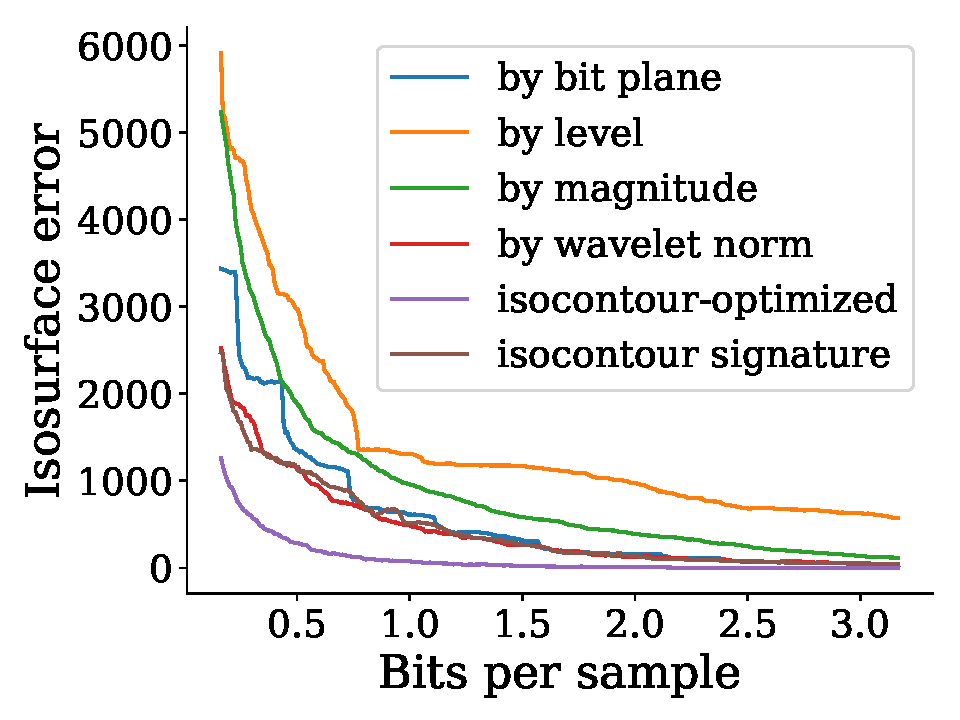
\includegraphics[width=0.48\linewidth]{isocontour/isocontour-optimized-pressure}}
	\subcaptionbox{turbulence}
	{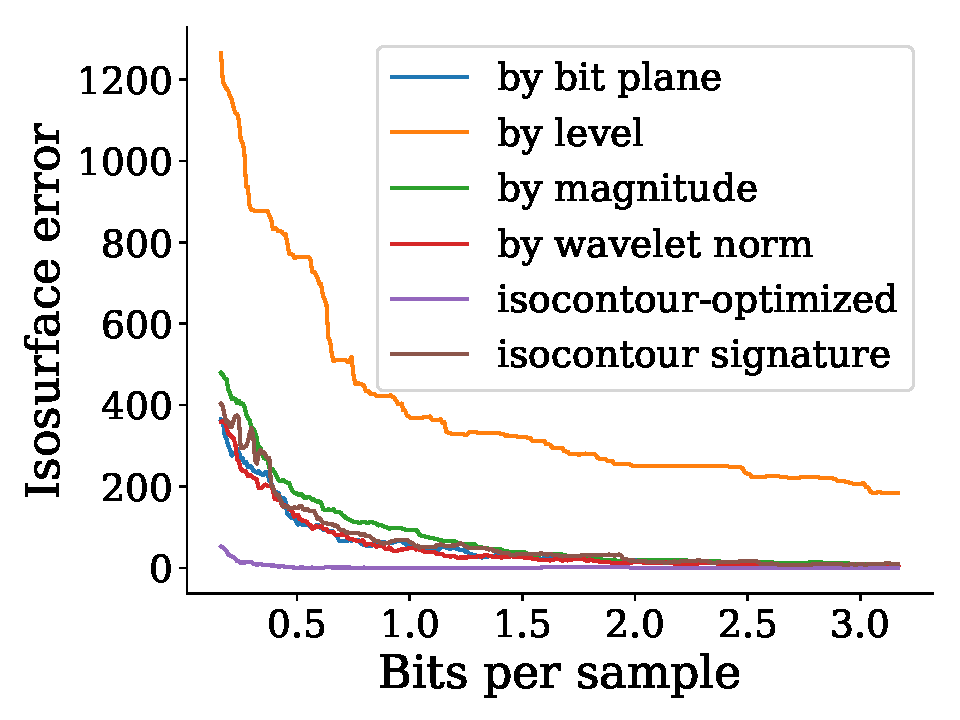
\includegraphics[width=0.48\linewidth]{isocontour/isocontour-optimized-turbulence}}
	\subcaptionbox{plasma}
	{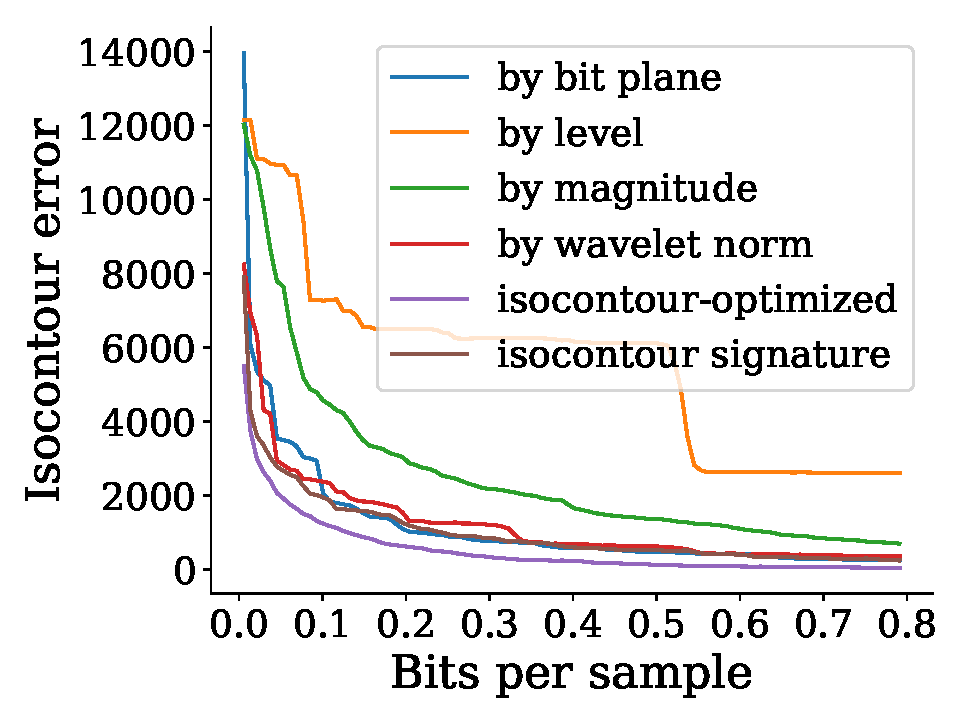
\includegraphics[width=0.48\linewidth]{isocontour/isocontour-optimized-plasma}}
	\subcaptionbox{diffusivity}
	{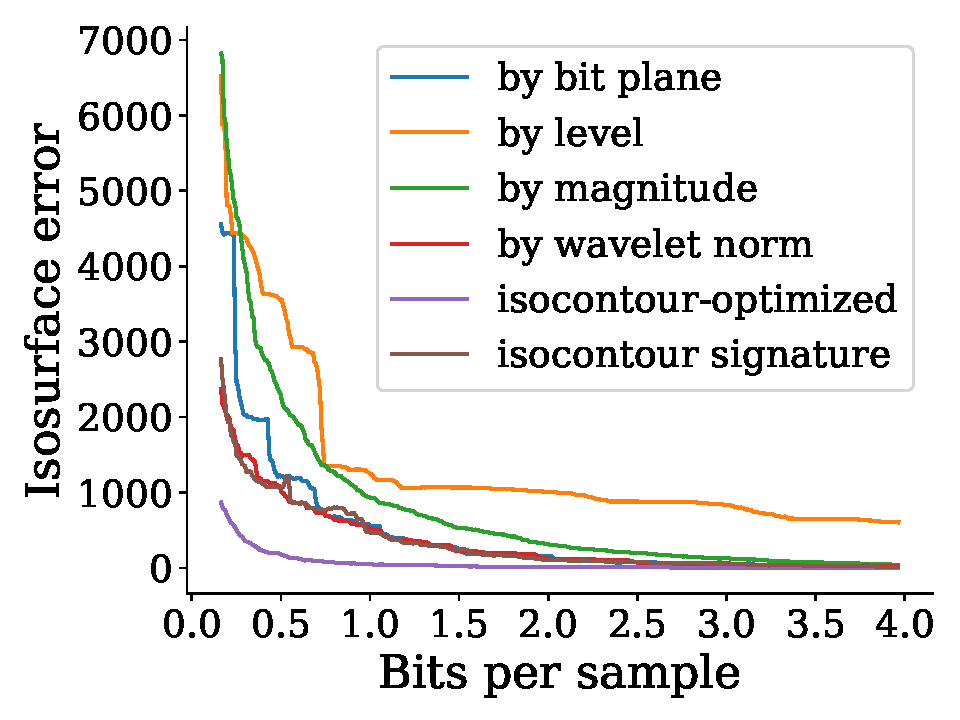
\includegraphics[width=0.48\linewidth]{isocontour/isocontour-optimized-diffusivity}}
	\caption{Isosurface errors for data-independent, \emph{isosurface-optimized}, and
                 {\em isosurface signature} streams. The bit rates are capped to highlight differences
                 among streams. The {\em by level} and {\em by magnitude} streams performs worst and the other remaining
                 streams have similar performance.}
	\label{fig:isocontour-plots}
\end{figure}

Qualitatively, we studied isosurfaces at specific bit rates for all streams. We were especially interested
at bit rates where the error is not exponentially decaying - the low bit rate isosurfaces do not resemble
the reference full data set isosurfaces. For example, at bit rate 0.4 the error curves are mostly flat and the gaps between
them result in isosurfaces with visible differences (\Cref{fig:isocontour-surfaces})).

\begin{figure}[h]
	\centering
	\subcaptionbox{\emph{by level}}
	{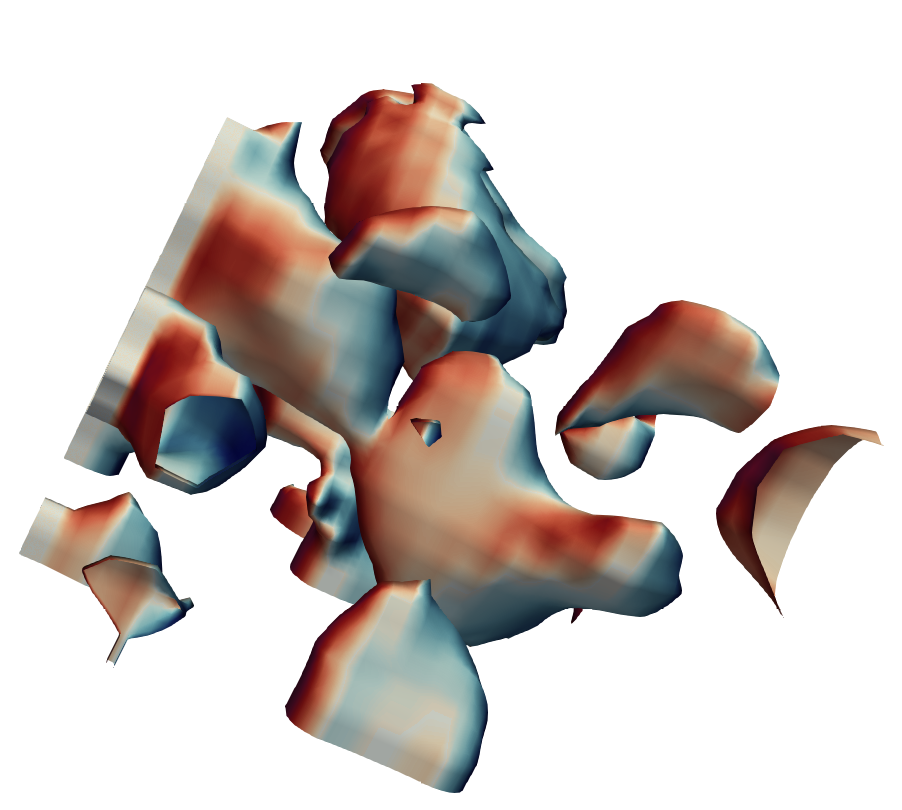
\includegraphics[width=0.31\linewidth]{isocontour/isocontour-pressure-level}}
	\subcaptionbox{\emph{by bit plane}}
	{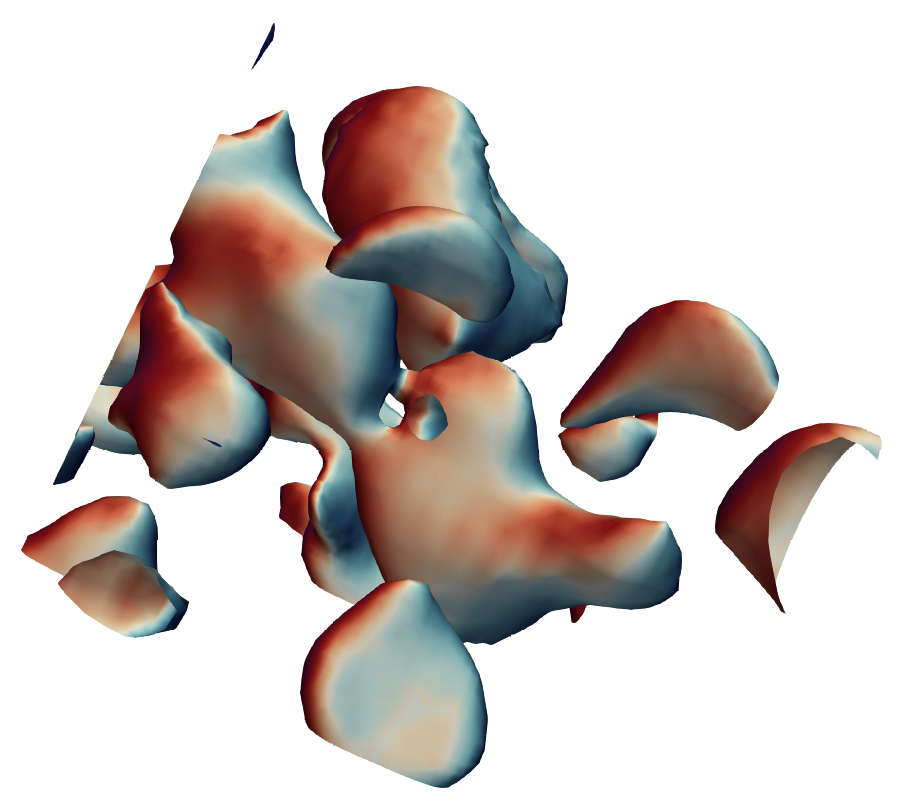
\includegraphics[width=0.31\linewidth]{isocontour/isocontour-pressure-bit-plane}}
	\subcaptionbox{\emph{by wavelet norm}}
	{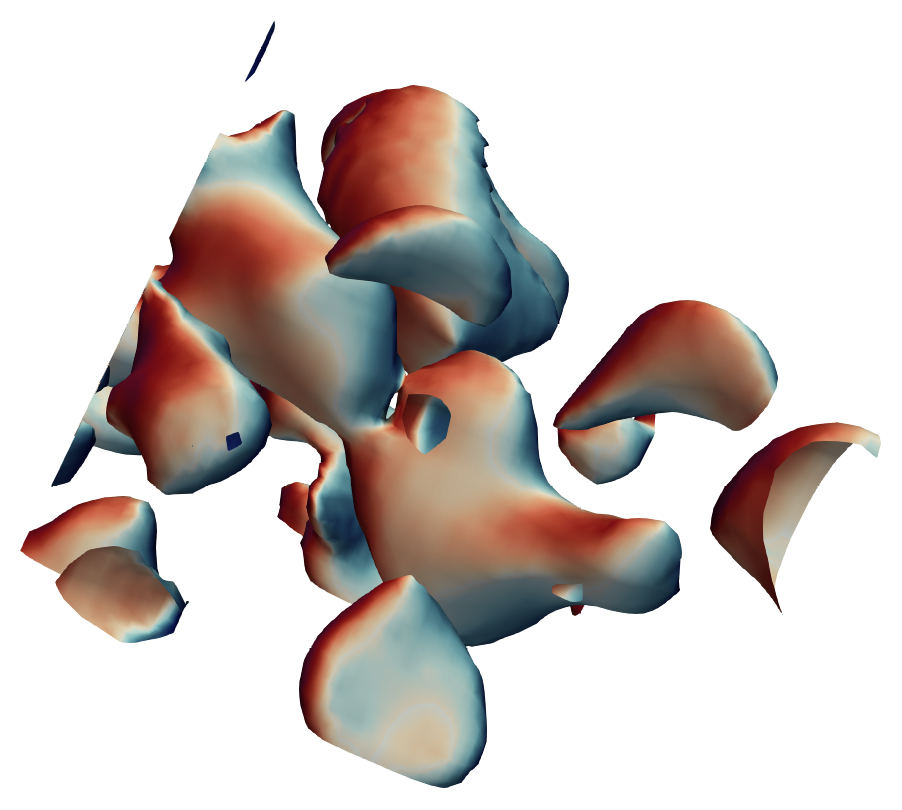
\includegraphics[width=0.31\linewidth]{isocontour/isocontour-pressure-wavelet-norm}}
	\subcaptionbox{\emph{by magnitude}}
	{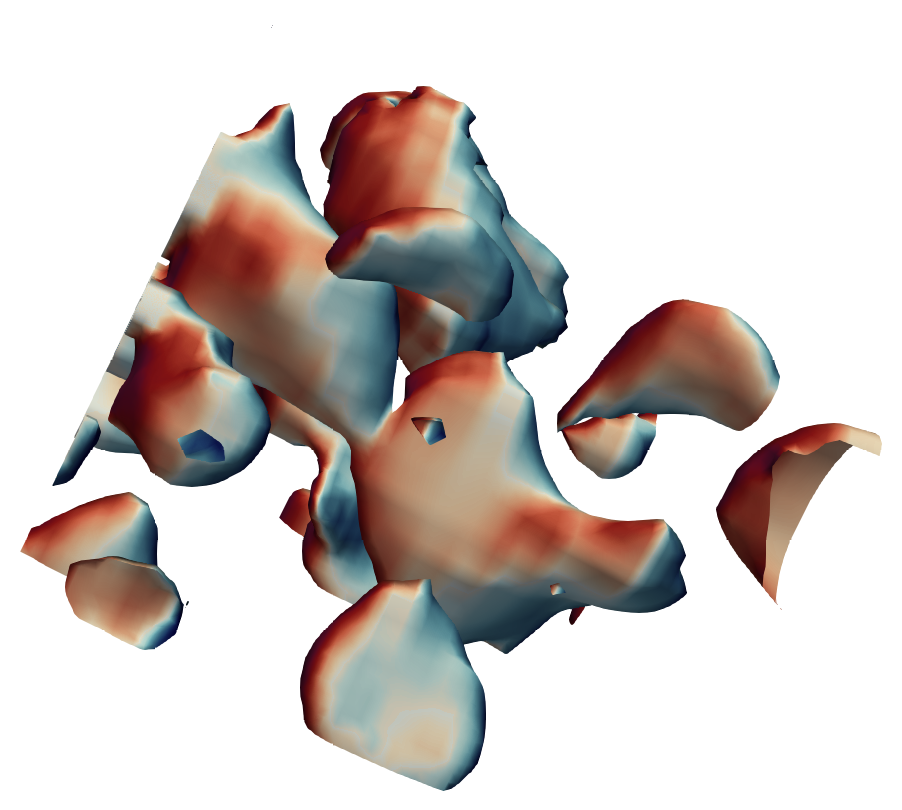
\includegraphics[width=0.31\linewidth]{isocontour/isocontour-pressure-magnitude}}
	\subcaptionbox{\emph{groundtruth}}
	{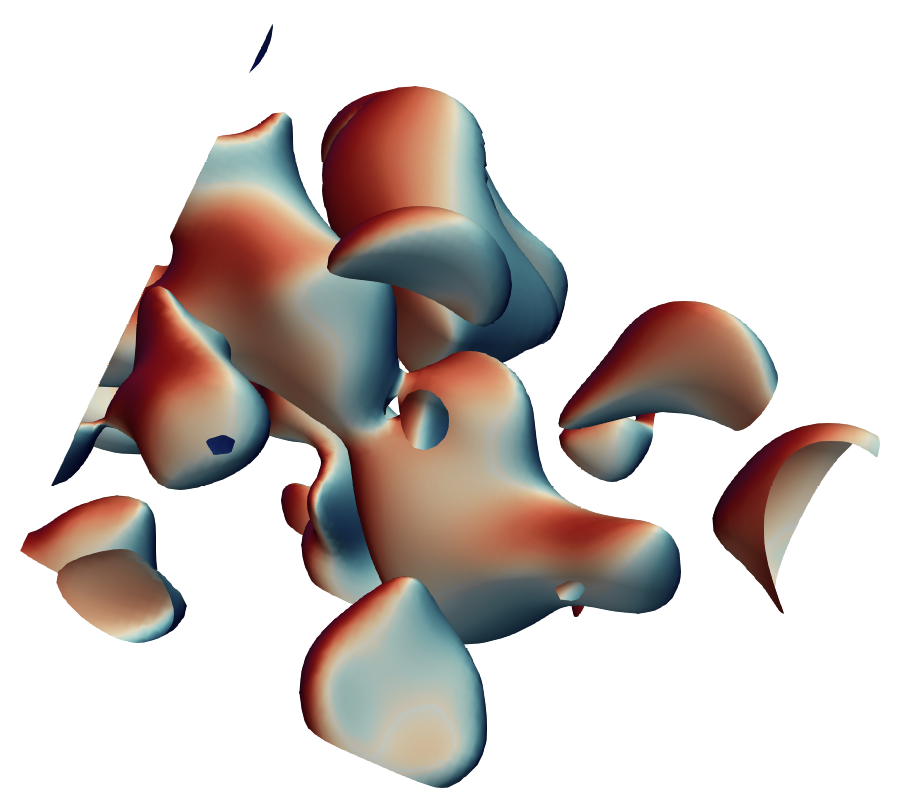
\includegraphics[width=0.31\linewidth]{isocontour/isocontour-pressure-groundtruth}}
	\caption{Miranda pressure field isosurfaces at bitrate of 0.4 bps.\pavol{what isovalue?} Both {\em by level}
        and {\em by magnitude} stream exhibit severe blocking artifacts compared to the groundtruth. The other streams
        still show smear artifacts, but the overall structure of the isosurfaces is more round and closer to the
        reference.}
	\label{fig:isocontour-surfaces}
\end{figure}

%Figure 5: We show that the hybrid and isocontour can diverge somewhat for low-gradient contour.
%Valerio suggested here we coudl also build a "ramp" dataset at different angles and see if the two
%diverges more as the ramp become flatter.

%We argue that if the gradient is low, some noise bits at the end will make an impact, the isocontour
%is very sensitive to noise, and is in general not interesting or meaninfgul to extract.


In this section, we looked at isosurface results for all six streams. The {\em by level} and {\em by magnitude} streams
show blocking artifacts compared to the less severe smearing of {\em by wavelet norm} and {\em by precisio} streams. Therefore,
it seems that one of those latter streams combined with a spatial adaptivity would perform well when isosurface
extraction is desired.
